\documentclass[11pt, a4paper]{article}

% --- Packages ---
\usepackage[utf8]{inputenc}
\usepackage{graphicx}
\usepackage[margin=0.8in]{geometry}
\usepackage{times}
\usepackage{xcolor}
\usepackage{titlesec}
\usepackage{enumitem}
\usepackage{float}
\usepackage{booktabs}
\usepackage{multirow}
\usepackage{amsmath}

% --- Amrita Colors ---
\definecolor{amritaMaroon}{HTML}{A4123F}

% --- Title & Section Formatting ---
\titlespacing*{\section}{0pt}{10pt}{3pt}
\titleformat{\section}{\large\bfseries\color{amritaMaroon}}{\thesection}{1em}{}

\pagestyle{empty}

\begin{document}

% ==========================================
% HEADER
% ==========================================
\noindent
\begin{minipage}{\textwidth}
\centering
{\Large \textbf{\textcolor{amritaMaroon}{
AMRITA VISHWA VIDYAPEETHAM \\
SCHOOL OF COMPUTING \\
DEPARTMENT OF COMPUTER SCIENCE AND ENGINEERING}}}

\vspace{0.2cm}

{\large \textbf{Explainable Federated Analytics for Multivariate Time-Series Forecasting with Personalized Drift Adaptation}}

\vspace{0.1cm}
23CSE399 -- Project Phase 1 (Panel Review 1)\\
\today
\end{minipage}

\vspace{0.3cm}
\hrule
\vspace{0.3cm}

% ==========================================
% TEAM DETAILS
% ==========================================
\begin{center}
\renewcommand{\arraystretch}{1.5}
\setlength{\tabcolsep}{5pt}
\begin{tabular}{|l|p{4.2cm}|p{4cm}|p{2.5cm}|c|}
\hline
\multicolumn{2}{|c|}{\textbf{Team Members}} & \textbf{Guide} & \textbf{Project Type} & \textbf{Marks} \\
\hline
CB.SC.U4CSE23547 & Sheela Akshar Sakhi &
\multirow{5}{=}{\raggedright \small \textbf{Dr. G R RAMYA, Dr. VANDHANA S}\\
\textit{Dept. of CSE}} &
\multirow{5}{=}{\raggedright \small \textbf{Type 1}\\Research} &
\multirow{5}{*}{\textbf{\huge \dots / 5}} \\ \cline{1-2}

CB.SC.U4CSE23529 & Hasini Reddy M & & & \\ \cline{1-2}
CB.SC.U4CSE23761 & Kousik Sarma Lakkaraju & & & \\ \cline{1-2}
CB.SC.U4CSE23363 & Haswitha K & & & \\ \cline{1-2}
CB.SC.U4CSE23753 & V.Chakravarthy & & & \\
\hline
\end{tabular}
\end{center}

\vspace{0.3cm}

% ==========================================
% 1. PROBLEM & ORIGINALITY
% ==========================================

\section{Problem Definition \& Originality}

\textbf{Problem Statement:}

Collaborative time-series forecasting across distributed organizations requires model training without centralizing sensitive data. Although Federated Learning enables privacy-preserving distributed training, existing systems fail to simultaneously address four critical challenges:

\begin{enumerate}[noitemsep]
\item Privacy preservation,
\item Client heterogeneity (non-IID distributions),
\item Concept drift in evolving environments,
\item Explainability of predictions.
\end{enumerate}

This limitation restricts trustworthy deployment in real-world domains such as healthcare analytics, smart grids, industrial IoT systems, and smart cities.

\vspace{0.2cm}

\textbf{Originality Claim (Extension-Based Research):}

This research extends classical Federated Averaging and Personalized Federated Learning frameworks by introducing:

\begin{itemize}[noitemsep]
\item A hybrid global–personalized architecture,
\item Online concept drift detection integrated within federated rounds,
\item Attention-based explainable forecasting,
\item Adaptive retraining triggered by statistical thresholds.
\end{itemize}

Unlike prior works that address these challenges independently, this study proposes a unified framework integrating personalization, drift adaptation, and explainability within a single federated architecture.

% ==========================================
% 2. LITERATURE SURVEY & GAP
% ==========================================

\section{Literature Survey \& Gap Analysis}

Federated Learning introduced decentralized training via weighted model aggregation. Later works introduced personalization layers to mitigate client heterogeneity. Drift detection has been studied primarily in centralized machine learning systems.

However, survey findings indicate:

\begin{itemize}[noitemsep]
\item Personalization improves accuracy but lacks interpretability.
\item Drift detection rarely operates within federated loops.
\item Explainable AI techniques are seldom integrated into federated time-series forecasting.
\item Multivariate time-series under federated settings remains under-explored.
\item Most studies assume static environments.
\end{itemize}

\textbf{Research Gap:}

There is no comprehensive federated framework that simultaneously provides:

\begin{itemize}[noitemsep]
\item Personalized learning for non-IID clients,
\item Online concept drift monitoring,
\item Attention-based explainable predictions,
\item Robust multivariate forecasting performance.
\end{itemize}

% ==========================================
% 3. PROPOSED METHODOLOGY
% ==========================================

\section{Proposed Methodology (Technical Knowledge)}

\textbf{Proposed Model: Federated Personalized Drift-Aware Attention Framework (FPDAF)}

The framework consists of three integrated modules:

\begin{enumerate}[noitemsep]
\item Global Shared Backbone for capturing common temporal dynamics.
\item Client-Specific Personalization Layers for local adaptation.
\item Drift-Aware Monitoring Module using statistical change detection.
\end{enumerate}

\textbf{Attention Mechanism:}

Temporal attention weights are computed as:

\[
\alpha_t = \frac{\exp(e_t)}{\sum_{k}\exp(e_k)}
\]

where $\alpha_t$ represents the importance of timestep $t$.

% ==========================================
% FIGURE
% ==========================================

\begin{figure}[H]
\centering
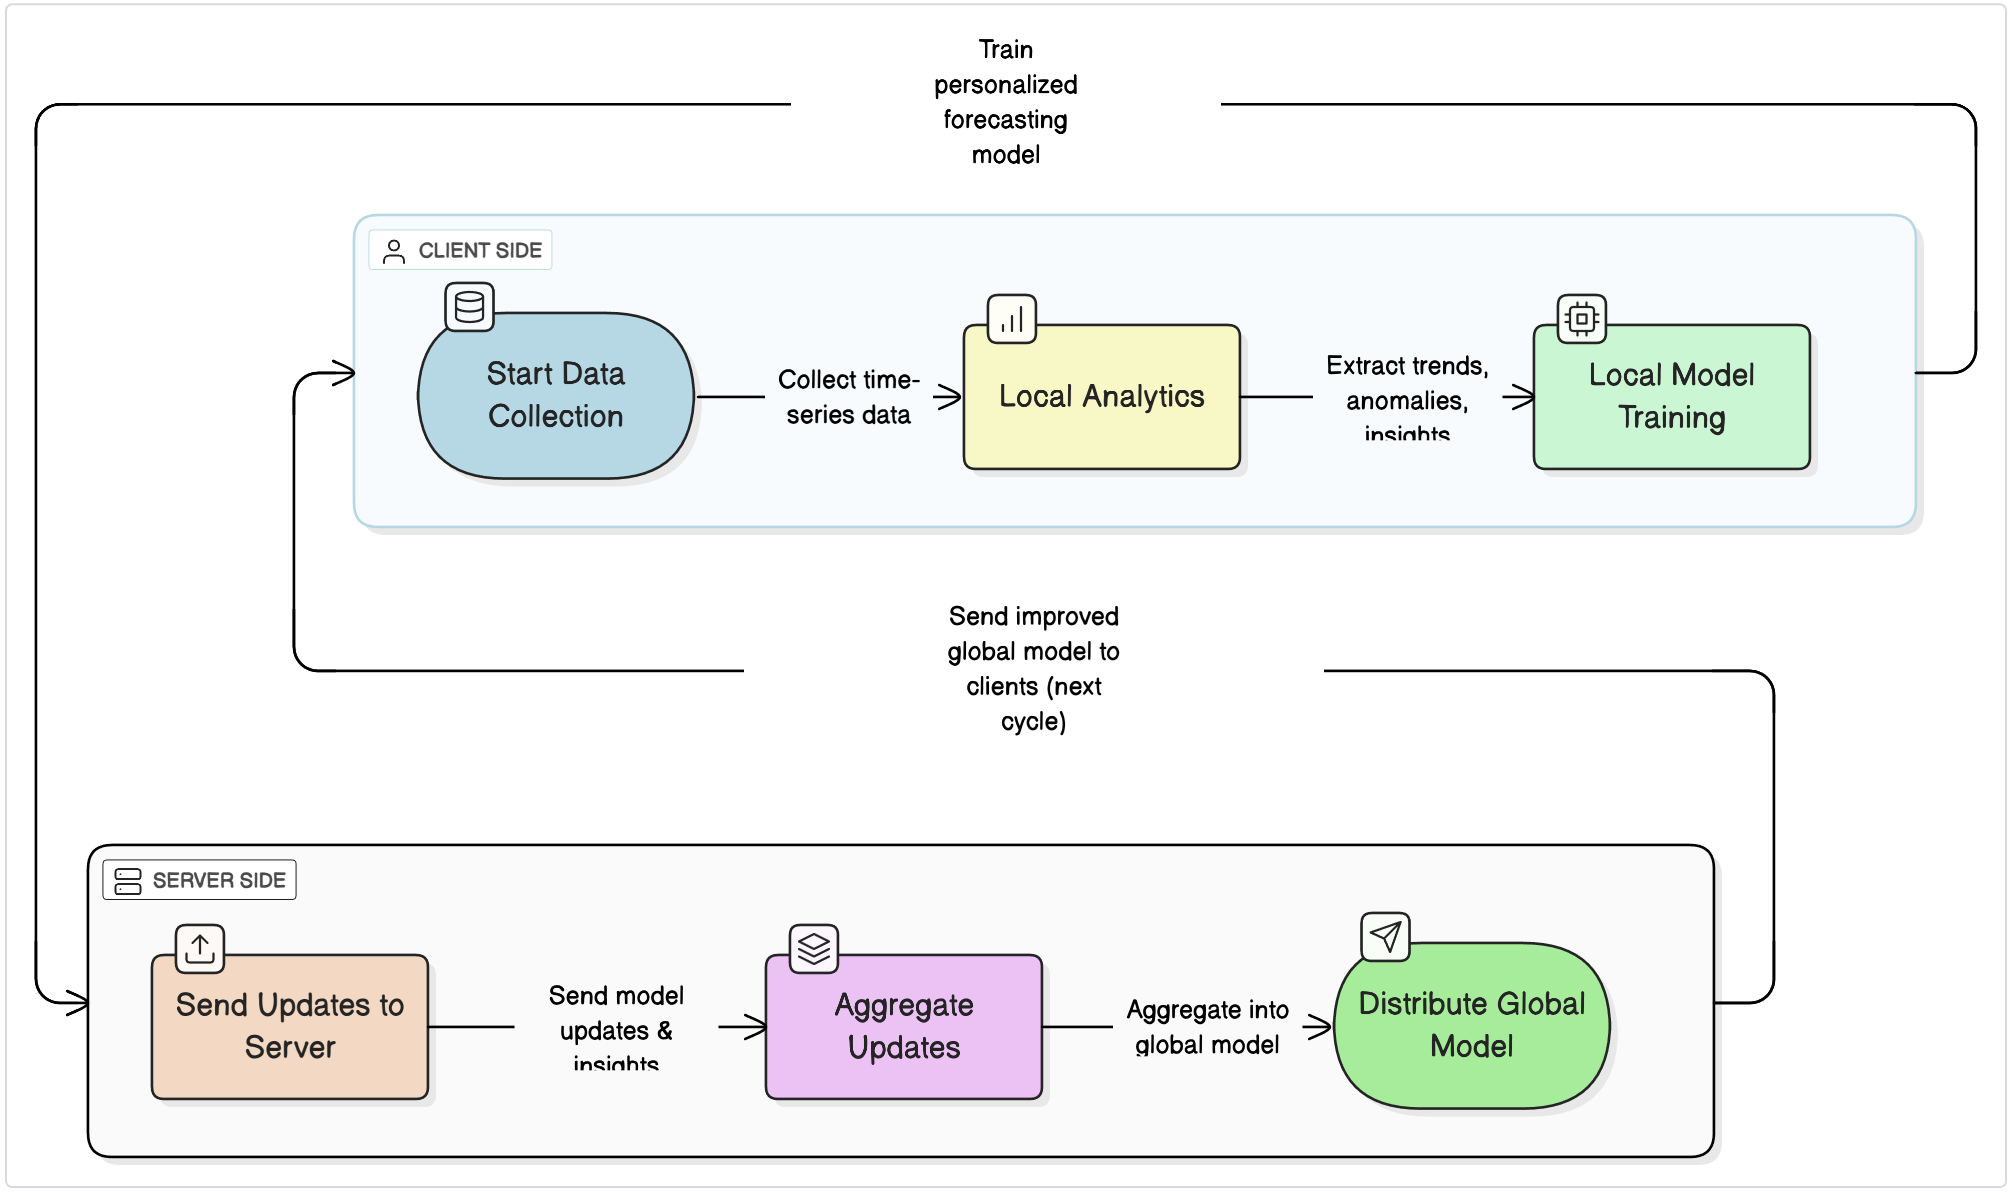
\includegraphics[width=0.85\linewidth]{AWF.png}
\caption{Adaptive Workflow Framework (AWF) illustrating federated personalization and drift adaptation pipeline}
\end{figure}


\vspace{0.2cm}
\begin{center}
\footnotesize
\textbf{Training Flow:} 
Local Training $\rightarrow$ Secure Upload $\rightarrow$ Global Aggregation $\rightarrow$ Model Redistribution
\end{center}

% ==========================================
% MATHEMATICAL BASIS
% ==========================================

\textbf{Federated Aggregation:}

\[
w^{t+1} = \sum_{i=1}^{N} \frac{n_i}{n} w_i^t
\]

\textbf{Concept Drift Detection (CUSUM):}

\[
S_t = \max(0, S_{t-1} + (x_t - \mu - k))
\]

If $S_t > h$, adaptive retraining is triggered.

% ==========================================
% 4. EVALUATION STRATEGY
% ==========================================

\section{Evaluation Strategy}

The framework will be evaluated using:

\begin{itemize}[noitemsep]
\item Prediction metrics: RMSE, MAE, MAPE.
\item Personalization gain over global FedAvg.
\item Drift responsiveness after distribution shift.
\item Explainability consistency via attention stability.
\end{itemize}

Baselines include:

\begin{itemize}[noitemsep]
\item Centralized LSTM/Transformer.
\item Standard Federated Averaging.
\item Non-personalized federated models.
\end{itemize}

% ==========================================
% 5. CURRENT STATUS & PLAN
% ==========================================

\section{Current Status \& Plan}

\textbf{Current Status:}

\begin{itemize}[noitemsep]
\item Literature survey of 25 peer-reviewed papers completed.
\item Research gap formalized.
\item Mathematical framework defined.
\item Architecture conceptualized.
\end{itemize}

\textbf{Next Steps:}

\begin{itemize}[noitemsep]
\item Implementation of personalized federated model.
\item Integration of drift detection module.
\item Multi-client simulation experiments.
\item Benchmarking and ablation study.
\end{itemize}

% ==========================================
% REFERENCES
% ==========================================

\nocite{*}
\renewcommand{\refname}{\normalsize References}
\bibliographystyle{IEEEtran}
\bibliography{ref}

\end{document}